\documentclass[crop,tikz]{standalone}

\usepackage[utf8]{inputenc}
% 'crop' is the default for v1.0, before it was 'preview'
%\usetikzlibrary{...}% tikz package already loaded by 'tikz' option
\usetikzlibrary{decorations.markings}

%The idea behind this file is that it will be used to store all the maths-related macros that I concoct; so that I can import all the commands by \input{this file} in the preamble of any file that I want to use them in.
%This should make the top-level files look a lot cleaner, and the preamble much shorter!

\usepackage{amssymb}
\usepackage{amsmath}

%theorems and lemma etc setup using amsthm
\usepackage{amsthm}
\newcommand{\tstk}[1]{\textbf{#1} \newline}
\theoremstyle{definition}
\newtheorem{definition}{Definition}[section]
\theoremstyle{plain}
\newtheorem{theorem}{Theorem}[section]
\theoremstyle{plain}
\newtheorem{lemma}[theorem]{Lemma}
\theoremstyle{plain}
\newtheorem{prop}[theorem]{Proposition}

\allowdisplaybreaks %allows equations in the same align environment to split over multiple pages.

%begin the macros via newcommand. Try to group them up reasonably!

%standard sets
\newcommand{\naturals}{\mathbb{N}}			%natural numbers
\newcommand{\integers}{\mathbb{Z}}			%integers
\newcommand{\rationals}{\mathbb{Q}}			%rational numbers
\newcommand{\reals}{\mathbb{R}}				%real numbers
\newcommand{\complex}{\mathbb{C}}			%complex numbers

%brackets and norms
\newcommand{\bracs}[1]{\left( #1 \right)}				%encloses input in brackets
\newcommand{\sqbracs}[1]{\left[ #1 \right]}				%encloses input in square brackets
\newcommand{\clbracs}[1]{\left\{ #1 \right\}}			%encloses input in curly bracers
\newcommand{\abs}[1]{\lvert #1 \rvert}					%absolute value
\newcommand{\norm}[2]{\lvert\lvert #1 \rvert\rvert}		%norm (double line)

%function sets
\newcommand{\smooth}[1]{C^{\infty}\bracs{#1}}							%smooth functions
\newcommand{\ltwo}[2]{L^{2}\bracs{#1,\mathrm{d}#2}}						%general L^2 space
\newcommand{\gradSob}[2]{H^1_\mathrm{grad}\bracs{#1, \mathrm{d}#2}}		%gradient Sobolev space
\newcommand{\curlSob}[2]{H^1_\mathrm{curl}\bracs{#1, \mathrm{d}#2}}		%curl Sobolev space
\newcommand{\kSob}[2]{H^1_{k,\mathrm{curl}}\bracs{#1, \mathrm{d}#2}}	%k-curl Sobolev space

%grad and curl sets
\newcommand{\gradZero}[2]{\mathcal{G}_{ #1, \mathrm{d}#2}\bracs{0}}		%gradients of zero for domain #1 with measure #2
\newcommand{\curlZero}[2]{\mathcal{C}_{ #1, \mathrm{d}#2}\bracs{0}}	%curls of zero for domain #1 with measure #2

%derivatives and grad-like symbols
\newcommand{\diff}[2]{\dfrac{\mathrm{d}#1}{\mathrm{d}#2}}			%complete derivative d#1/d#2
\newcommand{\pdiff}[2]{\dfrac{\partial #1}{\partial #2}}			%partial derivative p#1/p#2
\newcommand{\ddiff}[2]{\dfrac{\mathrm{d}^2 #1}{\mathrm{d}^2 #2}}	%2nd deriv
\newcommand{\grad}{\nabla}											%grad operator
\newcommand{\curl}[1]{\grad_{#1}\wedge}								%curl with measure subscript #1

%displaying integrals
\newcommand{\integral}[3]{\int_{#1}#2 \ \mathrm{d}#3}			%integral, domain #1, integrand #2, measure #3

%notation for variable use throughout the file
\newcommand{\dddom}{\widetilde{\Omega}}			%3D domain notation
\newcommand{\ddom}{\Omega}						%2D domain notation
\newcommand{\dddmes}{\widetilde{\mu}}			%3D measure
\newcommand{\ddmes}{\mu}						%2D measure

\newcommand{\graph}{\mathbb{G}}					%graph variable

%so as to be consistent with the photonic fibre picture, make sure that the image is no greater than a 5\times 5 size (plus text to one side I guess)

\begin{document}

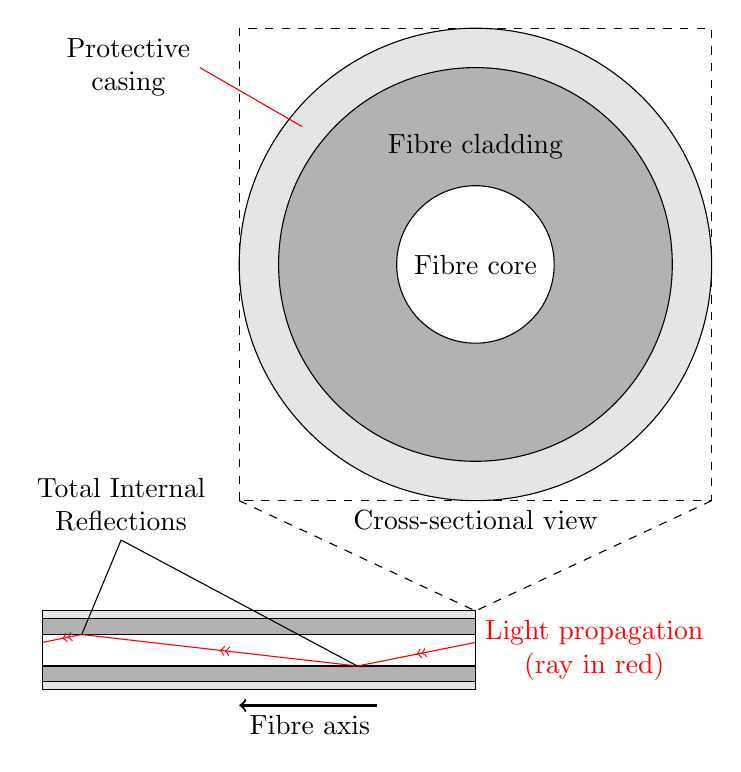
\begin{tikzpicture}
	%core, cladding, and casing plus labels
	\filldraw[fill=black!10!white, draw=black] (0,0) circle (3);       	
	\filldraw[fill=black!30!white, draw=black] (0,0) circle (2.5);
	\filldraw[fill=black!0!white, draw=black] (0,0) circle (1);
	\node[anchor=center] at (0,0) {Fibre core};
	\node[anchor=center] at (0,1.5) {Fibre cladding};
	\draw[red] (-2.2,1.75) -- (-3.5,2.5);
	\node[anchor=east, align=center] at (-3.5,2.5) {Protective \\ casing};
	%box to illustrate that this is the cross-section
	\draw[dashed] (-3,-3) rectangle (3,3);
	\draw[dashed] (-3,-3) -- (0,-4.4);
	\draw[dashed] (3,-3) -- (0,-4.4);
	\node[anchor=north, align=center] at (0,-3) {Cross-sectional view};

	%propagation mechanism, casing
	\begin{scope}[shift={(0,-1)}]
		\filldraw[fill=black!10!white, draw=black] (-5.5,-3.4) rectangle (0,-3.5);
		\filldraw[fill=black!30!white, draw=black] (-5.5,-3.5) rectangle (0,-3.7);
		\filldraw[fill=black!0!white, draw=black] (-5.5,-3.7) rectangle (0,-4.1);
		\filldraw[fill=black!30!white, draw=black] (-5.5,-4.1) rectangle (0,-4.3);
		\filldraw[fill=black!10!white, draw=black] (-5.5,-4.3) rectangle (0,-4.4);
		%light ray (yRange is -3.7 to -4.1), length is 5.5
		\begin{scope}[decoration={markings, mark=at position 0.5 with {\arrow{>>}}}]
			\draw[red, postaction=decorate] (0,-3.8) -- (-1.5,-4.1);
			\draw[red, postaction=decorate] (-1.5,-4.1) -- (-5,-3.7);
			\draw[red, postaction=decorate] (-5,-3.7) -- (-5.5,-3.8);
		\end{scope}
		%light ray labels
		\node[red, anchor=west, align=center] at (0,-3.9) {Light propagation \\ (ray in red)};
		%TIR points
		\draw[black] (-1.5,-4.1) -- (-4.5,-2.5);
		\draw[black] (-5,-3.7) -- (-4.5,-2.5);
		\node[anchor=south, align=center] at (-4.5,-2.5) {Total Internal \\  Reflections};
		%fibre axis for clarity
		\draw[->, thick] (-1.25, -4.6) -- (-3,-4.6) node[anchor=north west] {Fibre axis};
	\end{scope}

\end{tikzpicture}

\end{document}